\documentclass[tikz,border=10pt]{standalone}
\usetikzlibrary{shapes.geometric, positioning, arrows.meta, scopes, patterns, shadows, calc}
% I'll assume that the 'ez_utils' file provides additional utilities for your use. If not, please remove the line below.
\usepackage{xstring}

\def\code#1{\color{olive}{\texttt{#1}}\color{black}~}
% \def\refer#1{Fig. \ref{#1}}
% \newcommand{\urlpath}[1]{%
% \begin{FVerbatim}[fontsize=\scriptsize]
% #1
% \end{FVerbatim}%
% }

\def\comment#1{\color{olive}{\textit{\% #1}} \color{black}}

\newcommand\ezeq[1]{$#1$}

\newcommand\ezcolumn[3]{
\begin{column}{#1\textwidth}
    \vspace{#2cm}
    #3
\end{column}
}

% \newenvironment{myenumerate}{%
%   \begin{enumerate}
%     \renewcommand{\theenumii}{\arabic{enumi}.\arabic{enumii}}
%   }
%   {%
%   \end{enumerate}
% }


\newcommand{\customenumerate}{%
  \renewcommand{\theenumii}{\arabic{enumi}.\arabic{enumii}}
  \renewcommand{\theenumiii}{\arabic{enumi}.\arabic{enumii}.\arabic{enumiii}}
}


\begin{document}
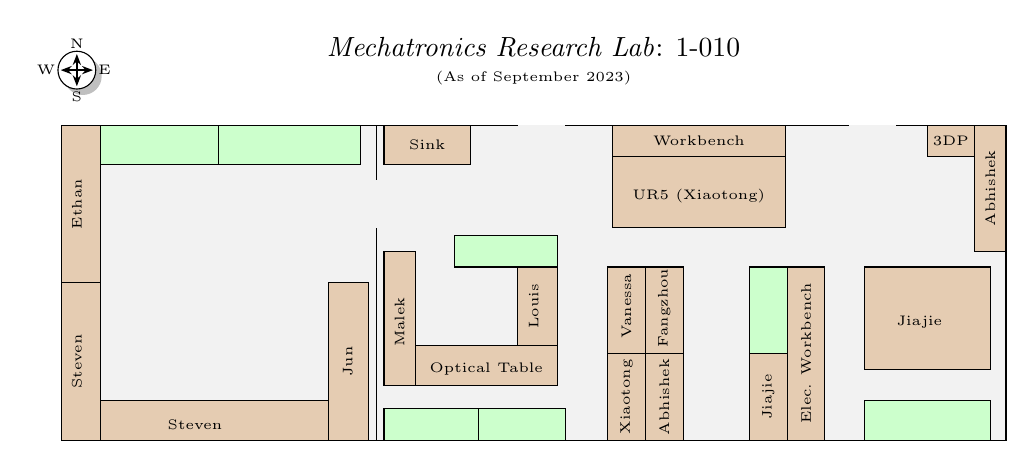
\begin{tikzpicture}[
    startstop/.style={rectangle, rounded corners, minimum width=3cm, minimum height=1cm, text centered, draw=green, fill=green!30, drop shadow},
    process/.style={rectangle, minimum width=3cm, minimum height=1cm, text centered, draw=black, fill=orange!30, drop shadow},
    io/.style={trapezium, trapezium left angle=70, trapezium right angle=110, minimum width=3cm, minimum height=1cm, text centered, draw=blue, fill=blue!30, drop shadow},
    decision/.style={diamond, minimum width=3cm, minimum height=1.5cm, text centered, draw=blue, fill=blue!30, drop shadow},
    arrow/.style={thick,->,>=stealth, shorten >=1pt},
]

% Drawing the lab space
\begin{scope}[scale=2]
    % At the top of the lab space, make a node text that says "Mechatronics Research Lab: 1-010"
    \node[font=\normalfont] at (3,2.5) {\textit{Mechatronics Research Lab}: 1-010};

    % Add a node under that says "Updated as of September 2023"
    \node[font=\tiny] at (3,2.3) {(As of September 2023)};


    % Drawing the lab's desk space (rectangle)
    \fill[fill=gray!10] (0,0) rectangle (6,2);  % 3:1 ratio as per your lab space dimensions.
    \draw (2.9,2) -- (0,2) -- (0,0) -- (6,0) -- (6,2) -- (5.3,2); % 3:1 ratio as per your lab space dimensions.
    \draw (5,2) -- (3.2,2); % 3:1 ratio as per your lab space dimensions.

    % At 2.5 units from the left, add a label that says Entrance 1
    % \node[font=\tiny] at (3,2.1) {Entrance 1};

    % At 5.5 units from the left, add a label that says Entrance 2
    % \node[font=\tiny] at (5.2,2.1) {Entrance 2};

    % Drawing the box with a door cutout
    \draw[fill=gray!10] (0,0) rectangle (2,2); % This creates a box with a door cutout near the top.
    \fill[fill=gray!10] (1.9,1.35) rectangle (2.2,1.65); % This creates the door cutout.

    % Draw the sink right next to entracne 1
    \draw[fill=brown!40] (2.05,1.75) rectangle (2.6,2);

    % Label the sink with a tiny font and situate it vertically
    \node[font=\tiny] at (2.325,1.875) {Sink};

    % Draw a box in the bottom left corner for Steven's desk/workspace
    \draw[fill=brown!40] (0,0) rectangle (0.25,1);
    \draw[fill=brown!40] (0.25,0) rectangle (1.7,0.25);

    % Label Steven's desk/workspace with a tiny font and situate it vertically
    \node[font=\tiny, rotate=90] at (0.1,0.5) {Steven};

    % Label his works pace with a tiny font and situate it horizontally
    \node[font=\tiny] at (0.85,0.1) {Steven};

    % Draw a box in the bottom right corner for Jun's workspace
    \draw[fill=brown!40] (1.95,0) rectangle (1.7,1);

    % Label Jun's workspace with a tiny font and situate it vertically
    \node[font=\tiny, rotate=90] at (1.82,0.5) {Jun};

    % Draw a box above steven's left most desk to the top of the lab space
    \draw[fill=brown!40] (0,1) rectangle (0.25,2);

    % Label the box as "Ethan" and situate it vertically
    \node[font=\tiny, rotate=90] at (0.1,1.5) {Ethan};

    % Draw a horizontal desk at the top of the lab space next to Ethan's desk that is the same width as Steven's workspace
    \draw[fill=green!20] (0.25,1.75) rectangle (1,2);

    % Draw another horizontal desk next to the previous one that is ~1 units wide
    \draw[fill=green!20] (1,1.75) rectangle (1.9,2);

    % Draw a vertical desk to the right of Jun's desk that is the same height as Jun's desk
    \draw[fill=brown!40] (2.05,0.35) rectangle (2.25,1.2);

    % Label this desk as "Malek" and situate it vertically
    \node[font=\tiny, rotate=90] at (2.15,0.75) {Malek};

    % Draw a horizontal desk whose left edge starts at the same left edge as Malek's desk and is the same width as Steven's desk
    \draw[fill=green!20] (2.5,1.1) rectangle (3.15,1.3);

    % Draw a vertical desk with width of 0.2 units to the right of the previous desk
    \draw[fill=brown!40] (2.9,1.1) rectangle (3.15,0.6);

    % Label this desk as "Louis" and situate it vertically
    \node[font=\tiny, rotate=90] at (3,0.85) {Louis};

    % Draw a horizontal desk parallel to one of the green ones
    \draw[fill=brown!40] (2.25,0.6) rectangle (3.15,0.35);

    % Label as "Optical Table" and horizontal
    \node[font=\tiny] at (2.7,0.45) {Optical Table};

    % Draw a horizontal desk whose left edge starts at the same left edge as Malek's desk and is the same width as Steven's desk
    \draw[fill=green!20] (2.05,0) rectangle (2.65,0.2);

    % Draw a horizontal desk next to this one same size
    \draw[fill=green!20] (2.65,0) rectangle (3.2,0.2);

    % Between the two entrances, draw a horizontal square whose top edge is the same as the top edge of the lab space
    \draw[fill=brown!40] (3.5,1.8) rectangle (4.6,2);

    % Label it as the workbench area and situate it horizontally
    \node[font=\tiny] at (4.05,1.9) {Workbench};

    % Directly underneath the workbench area, draw a horizontal desk that is the same width as the workbench area
    \draw[fill=brown!40] (3.5,1.8) rectangle (4.6,1.35);
    
    % Label it as the UR5 area and situate it horizontally
    \node[font=\tiny] at (4.05,1.55) {UR5 (Xiaotong)};

    % Create a group for the desks in the middle of the lab space
    \begin{scope}[shift={(-0.85,0.)}, xscale=1.2]
        % Between the two entrances, draw a vertical desk that is the same height as Jun's desk
        \draw[fill=brown!40] (3.6,0.55) rectangle (3.8,1.1);

        % Label it as Vanessa and situate it vertically
        \node[font=\tiny, rotate=90] at (3.7,0.85) {Vanessa};

        % Draw another identical desk right beneath hers
        \draw[fill=brown!40] (3.6,0.55) rectangle (3.8,0);

        % Label it as Xiaotong
        \node[font=\tiny, rotate=90] at (3.7,0.275) {Xiaotong};

        % Draw a vertical desk to the right of Xiaotong's desk that is the same height as Jun's desk
        \draw[fill=brown!40] (3.8,0.55) rectangle (4.,1.1);

        % Label this desk as Fangzhou and situate it vertically
        \node[font=\tiny, rotate=90] at (3.9,0.84) {Fangzhou};

        % Draw another identical desk right beneath hers
        \draw[fill=brown!40] (3.8,0.55) rectangle (4.,0);

        % Label it as Abhishek
        \node[font=\tiny, rotate=90] at (3.9,0.275) {Abhishek};

        % Draw a vertical desk to the right of Fangzhou's desk that is the same height as Jun's desk
        \draw[fill=green!20] (4.35,0.55) rectangle (4.55,1.1);

        % Draw another identical desk right beneath hers
        \draw[fill=brown!40] (4.35,0.55) rectangle (4.55,0);

        % Label it as "Jiajie" and situate it vertically
        \node[font=\tiny, rotate=90] at (4.45,0.275) {Jiajie};

        % Draw a vertical desk to the right of Jiajie's desk that is the same height as Jun's desk
        \draw[fill=brown!40] (4.55,0) rectangle (4.75,1.1);

        % Label it as "Electrical Workbench" and situate it vertically
        \node[font=\tiny, rotate=90] at (4.65,0.55) {Elec. Workbench};
    \end{scope}

    % Draw a vertical desk to the right of Jiajie's desk that is the same height as Jun's desk
    \draw[fill=brown!40] (5.1,0.45) rectangle (5.9,1.1);

    % Label it as Jiajie and situate it horizontally
    \node[font=\tiny] at (5.45,0.75) {Jiajie};


    % Draw a horizontal desk below
    \draw[fill=green!20] (5.1,0) rectangle (5.9,0.25);

    % Draw a vertical desk to the right of Jiajie's desk that is the same height as Jun's desk
    \draw[fill=brown!40] (5.8,1.2) rectangle (6,2);

    % Label it as Abhishek and situate it vertically
    \node[font=\tiny, rotate=90] at (5.9,1.6) {Abhishek};
    
    % Draw a horizontal desk below
    \draw[fill=brown!40] (5.5,1.8) rectangle (5.8,2);

    % Label it as 3DP
    \node[font=\tiny] at (5.65,1.9) {3DP};

    
\end{scope}

% Drawing the compass at the top right
\begin{scope}[shift={(0.2,4.7)},scale=0.3, font=\tiny]
    \draw[fill=white, drop shadow] (0,0) circle (0.8cm);
    \draw[arrow, >={Stealth[scale=0.6]}] (0,0) -- (0,0.8); % North with slightly bigger arrowhead
    \draw[arrow, >={Stealth[scale=0.6]}] (0,0) -- (0,-0.8); % South
    \draw[arrow, >={Stealth[scale=0.6]}] (0,0) -- (0.8,0); % East
    \draw[arrow, >={Stealth[scale=0.6]}] (0,0) -- (-0.8,0); % West
    \node[above] at (0,0.5) {N};
    \node[below] at (0,-0.5) {S};
    \node[right] at (0.5,0) {E};
    \node[left] at (-0.5,0) {W};
\end{scope}

\end{tikzpicture}
\end{document}
